\documentclass[tikz,border=10pt]{standalone}
\usepackage{tikz}
\usepackage{amsmath}
\usepackage{amssymb}  % For \mathbb
\usetikzlibrary{shapes,arrows,positioning,fit,backgrounds,matrix,decorations.pathreplacing}

\begin{document}
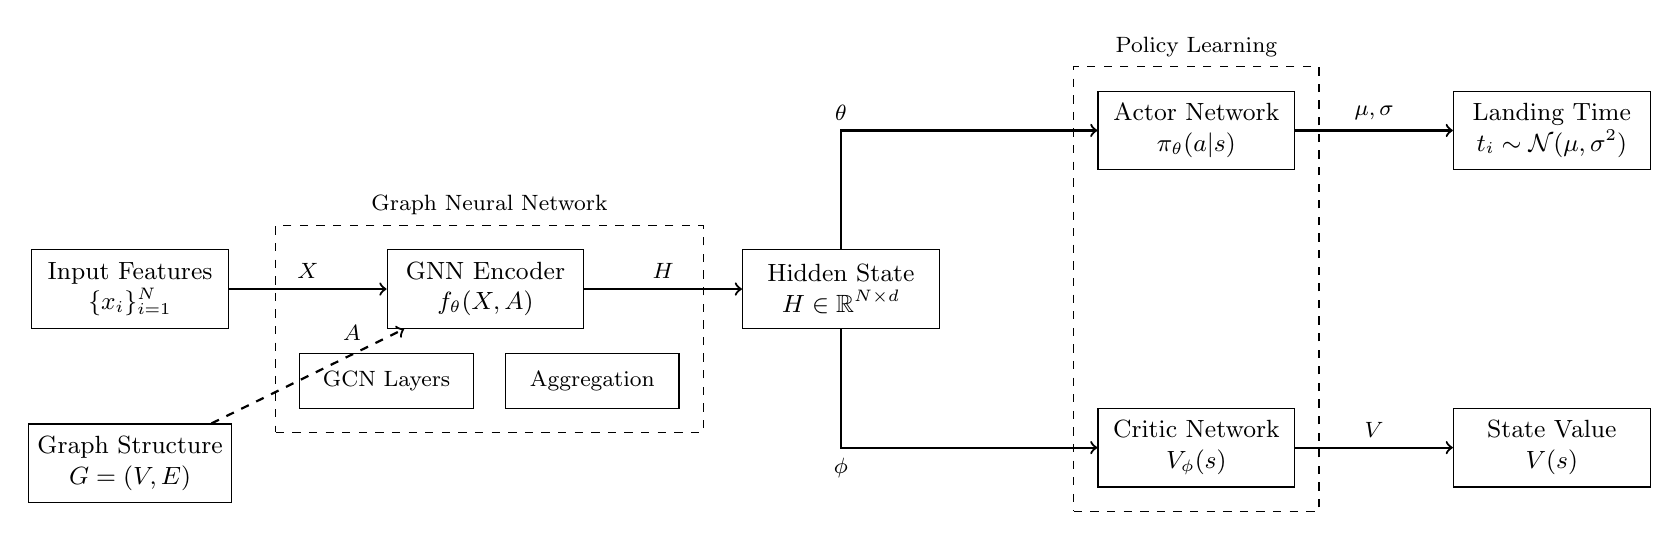
\begin{tikzpicture}[
    scale=1.0,  % Increase scale for better spacing
    node distance=2.5cm,  % Increase node distance
    box/.style={rectangle,draw,minimum width=2.5cm,minimum height=1cm,font=\small,align=center},
    feature/.style={rectangle,draw,minimum width=2.2cm,minimum height=0.7cm,font=\footnotesize},  % Adjust feature box size
    arrow/.style={->,thick},
    doublearrow/.style={<->,thick}
]
% Input Layer with Details
\node[box] (input) {Input Features\\$\{x_i\}_{i=1}^N$};
%\node[feature, below=0.3cm of input] (feat1) {Time Windows};
%\node[feature, below right=0.3cm and 0.2cm of input] (feat2) {Aircraft Cat.};
%\node[feature, below right=0.8cm and 0.2cm of input] (feat3) {Cost Coef.};
\node[box, below=1.2cm of input] (graph) {Graph Structure\\$G=(V,E)$};

% GNN Encoder
\node[box, right=2cm of input] (gnn) {GNN Encoder\\$f_{\theta}(X,A)$};
\node[feature, below=0.3cm of gnn.south west] (gnn1) {GCN Layers};
\node[feature, right=0.4cm of gnn1] (gnn2) {Aggregation};

% Hidden Representation
\node[box, right=2cm of gnn] (hidden) {Hidden State\\$H \in \mathbb{R}^{N \times d}$};

% Actor-Critic Heads
\node[box, above right=1cm and 2cm of hidden] (actor) {Actor Network\\$\pi_{\theta}(a|s)$};
\node[box, below right=1cm and 2cm of hidden] (critic) {Critic Network\\$V_{\phi}(s)$};

% Outputs
\node[box, right=2cm of actor] (action) {Landing Time\\$t_i \sim \mathcal{N}(\mu,\sigma^2)$};
\node[box, right=2cm of critic] (value) {State Value\\$V(s)$};

% Connections
\draw[arrow] (input) -- node[above,font=\footnotesize] {$X$} (gnn);
\draw[arrow, dashed] (graph) -- node[above right=0.45cm,font=\footnotesize] {$A$} (gnn);
\draw[arrow] (gnn) -- node[above,font=\footnotesize] {$H$} (hidden);
\draw[arrow] (hidden) |- node[above,font=\footnotesize] {$\theta$} (actor);
\draw[arrow] (hidden) |- node[below,font=\footnotesize] {$\phi$} (critic);
\draw[arrow] (actor) -- node[above,font=\footnotesize] {$\mu,\sigma$} (action);
\draw[arrow] (critic) -- node[above,font=\footnotesize] {$V$} (value);

% Background boxes for modules
\begin{pgfonlayer}{background}
    \node[rectangle,draw,dashed,fit=(gnn) (gnn1) (gnn2),inner sep=0.3cm,
          label=above:{\footnotesize Graph Neural Network}] {};
    \node[rectangle,draw,dashed,fit=(actor) (critic),inner sep=0.3cm,
          label=above:{\footnotesize Policy Learning}] {};
\end{pgfonlayer}

\end{tikzpicture}
\end{document}
